% !TeX program = xelatex
% Standalone English short communication; all content counts toward 10 pages.
\makeatletter\def\input@path{{./}{template/}}\makeatother
\documentclass[a4paper,12pt,review]{cas-sc}
% The supplied class hard-codes a 192 x 262 mm sheet. Set paper only;
% preserve its margins, fonts, captions, equation alignment and other styles.
\geometry{a4paper}
\usepackage[numbers,sort&compress]{natbib}
\usepackage{bm,algorithm,algpseudocode,placeins}
\newcommand{\R}{\mathbb R}
\newcommand{\C}{\mathbb C}
\newcommand{\Rea}{\operatorname{Re}}
\begin{document}
\let\WriteBookmarks\relax
\shorttitle{Variable-projection curvature for wideband direct positioning}
\shortauthors{B. Hao et al.}
\title[mode=title]{Variable-Projection Curvature for Efficient Newtonized Refinement in Wideband Direct Position Determination}
%% Author 1: Benjian Hao
\author[inst1]{Benjian Hao}[orcid=0000-0002-6676-7306]
\ead{bjhao@xidian.edu.cn}
% TODO(CRediT): Add \credit{...} after all authors approve their roles.
%% Author 2: Xinlei Wang
\author[inst1]{Xinlei Wang}[orcid=0000-0002-6855-3686]
\ead{wangxinlei@stu.xidian.edu.cn}
% TODO(CRediT): Add \credit{...} after all authors approve their roles.
%% Author 3: Zan Li (corresponding author)
\author[inst1]{Zan Li}[orcid=0000-0002-5207-6504]
\cormark[1]
\ead{zanli@xidian.edu.cn}
% TODO(CRediT): Add \credit{...} after all authors approve their roles.
\cortext[cor1]{Corresponding author.}
\affiliation[inst1]{organization={State Key Laboratory of Integrated Service Networks, School of Telecommunications Engineering, Xidian University},
  city={Xi'an},
  postcode={710071},
  country={China}}
% Funding and other unconfirmed metadata are left blank.
\begin{abstract}
Unknown wideband waveforms couple source positions to many frequency coefficients in direct position determination. Block Newtonized orthogonal matching pursuit reduces the search dimension, but position updates based on fixed coefficients can make slow progress even when waveforms are re-estimated during acceptance. We develop a variable-projection curvature update for this local refinement. Eliminating the current source coefficients removes a positive-semidefinite coupling term from the position Hessian; local analysis explains how this term can slow convergence. Frequency-wise accumulation requires only small matrices. In 240 paired two-source observations, replacing fixed-coefficient curvature under the same waveform-eliminated acceptance objective reduces mean complete runtime by 83.77\%, with identical success/failure decisions at a 20 m tolerance and no deterioration in terminal joint fitting or stationarity. A further 480-observation test distinguishes this local efficiency gain from the configuration sensitivity of the complete sequential locator. The method improves the computational efficiency of block refinement without changing residual-based source discovery.
\end{abstract}
\begin{keywords}
Direct position determination\sep Variable projection\sep Newton refinement\sep Unknown waveforms\sep Block orthogonal matching pursuit
\end{keywords}
\maketitle

\section{Introduction}
Direct position determination (DPD) fits synchronized receiver observations jointly to estimate emitter positions, avoiding intermediate delay association \cite{ChenHudsonYao2002,WeissAmar2005}. For overlapping unknown waveforms, positions and frequency coefficients must be estimated together. Sequential source discovery reduces the spatial search, but its cost can be dominated by repeated local refinement.

Newtonized orthogonal matching pursuit (NOMP) alternates discovery, Newton refinement and cyclic feedback \cite{Mamandipoor2016}. Gains are estimated during detection, updated during refinement and jointly refitted by least squares; the Newton direction nevertheless treats the current gain as fixed. Multi-frequency block NOMP extends this construction to two-dimensional positions and unknown source coefficients at each frequency \cite{Yang2022}. Its fixed-coefficient position derivatives provide the closest refinement reference. QNOMP uses joint quasi-Newton refinement and gain re-estimation for delay and angle parameters in pilot-based channel estimation \cite{Zeng2025}.

We retain block-NOMP discovery and cyclic updates, but account for the variation of the optimal waveform coefficients with position in the Newton curvature itself. Using classical variable projection \cite{GolubPereyra1973}, we derive an explicit frequency-wise correction for the wideband DPD response and relate it to slow local progress under position--waveform coupling. Small-matrix accumulation keeps the per-step cost linear in the number of frequencies. A controlled comparison uses the same waveform-eliminated acceptance objective and numerical safeguards to isolate the effect of curvature on the subsequent iterations and complete runtime. The contribution is this block-refinement construction and its mechanism-based validation, rather than gain re-estimation alone.

\section{Model and local objective}
Let $\bm r_l\in\R^2$ and $\bm p_k\in\Omega\subset\R^2$ denote station $l$ and source $k$. For $L$ synchronized single-antenna stations and known source count $K$, the retained DFT observations satisfy
\begin{equation}
 \bm x_f=\sum_{k=1}^K\bm a_f(\bm p_k)s_{k,f}+\bm n_f,
 \qquad [\bm a_f(\bm p)]_l=\frac{\exp[-\mathrm j2\pi f d_l(\bm p)/c_0]}{d_l(\bm p)},
 \label{eq:model}
\end{equation}
where $d_l(\bm p)=\|\bm p-\bm r_l\|$, $c_0$ is propagation speed, $f\in\mathcal F$ is signed baseband frequency, and $F=|\mathcal F|$. The unknown $s_{k,f}\in\C$ includes transmitted power. The known relative amplitude follows free-space loss; its common wavelength factor is absorbed into $s_{k,f}$ \cite{ITURP5252024}. We use a static, calibrated, direct-path baseband-delay model, without RF carrier phase or random link gains. The common-window approximation neglects station-dependent record edges \cite{ChenHudsonYao2002}. Independent complex Gaussian sample noise of variance $\sigma_t^2$ has retained-bin variance $\sigma_t^2/N$ for a $1/N$-normalized DFT of length $N$. Numerical evaluation floors distances at 1 m; the following smooth derivatives apply outside that protection region.

Write $E=\sum_f\|\bm x_f\|^2>0$. During refinement of source $j$, hold the other fitted contributions fixed and form $\bm y_f=\bm x_f-\sum_{k\ne j}\bm a_f(\bm p_k)\widehat s_{k,f}$. For trial position $\bm z\in\R^2$,
\begin{align}
 \mathcal L(\bm z,\bm q)&=E^{-1}\sum_f\|\bm y_f-\bm a_f(\bm z)q_f\|^2,
 &\widehat q_f(\bm z)&=\frac{\bm a_f^H\bm y_f}{\bm a_f^H\bm a_f},\label{eq:ls}\\
 \phi(\bm z)&=\min_{\bm q}\mathcal L(\bm z,\bm q)
 =E^{-1}\sum_f\left(\|\bm y_f\|^2-\frac{|\bm a_f^H\bm y_f|^2}{\bm a_f^H\bm a_f}\right).
 \label{eq:profile}
\end{align}
Here $\bm x_f,\bm y_f,\bm n_f\in\C^L$ and $\bm q\in\C^F$. Superscripts $H$ and $T$ denote conjugate and ordinary transpose; $\mathrm j^2=-1$ and $I_2$ is the identity. All current-source coefficients are eliminated; the other source contributions remain fixed within this local call.

\section{Waveform-eliminated curvature}
At the current position, set $q_f=\widehat q_f$, $\bm e_f=\bm y_f-\bm a_fq_f$, and define $\bm a_{f,i}=\partial\bm a_f/\partial z_i$ and $\bm a_{f,ij}=\partial^2\bm a_f/\partial z_i\partial z_j$. Differentiating with fixed coefficients gives
\begin{align}
 g_i&=-\frac{2}{E}\Rea\sum_f\bm e_f^H\bm a_{f,i}q_f,\label{eq:g}\\*
 [H_{zz}]_{ij}&=\frac{2}{E}\Rea\sum_f
 \left(|q_f|^2\bm a_{f,i}^H\bm a_{f,j}-\bm e_f^H\bm a_{f,ij}q_f\right).
 \label{eq:hfixed}
\end{align}
Coefficient optimality makes $\bm g$ also the gradient of $\phi$, but $H_{zz}$ is not its Hessian. To obtain the reduced Hessian, collect coefficient real and imaginary parts in $\bm u\in\R^{2F}$. Differentiating $\nabla_u\mathcal L(\bm z,\widehat{\bm u}(\bm z))=0$ gives
\begin{equation}
 \frac{\partial\widehat{\bm u}}{\partial\bm z}=-H_{uu}^{-1}H_{uz},\qquad
 H_{\rm VP}=H_{zz}-H_{zu}H_{uu}^{-1}H_{uz}.
 \label{eq:schur}
\end{equation}
Here $H_{\rm VP}$ is the Hessian of the conditional local objective $\phi$: only the current source coefficients are eliminated, with all other fitted contributions fixed. It is not the Hessian of the full jointly concentrated position objective. This standard elimination identity \cite{GolubPereyra1973} requires a smooth response and a locally unique coefficient minimizer. All blocks are evaluated at the current coefficient optimum. Here $H_{uu}$ is block diagonal with $2\times2$ blocks $2\|\bm a_f\|^2 I_2/E$, so it is positive definite. Consequently, $H_{zz}-H_{\rm VP}\succeq0$: fixed-coefficient curvature includes response changes that waveform adjustment can compensate.

For explicit evaluation, let $\bm D_f=[\bm a_{f,1},\bm a_{f,2}]$, $\bm c_f=q_f(\bm a_f^H\bm D_f)^T$ and $\bm b_f=(\bm e_f^H\bm D_f)^T$. The mixed block for frequency $f$ is
\begin{equation}
 H_{zu,f}=\frac{2}{E}
 [\Rea(\bm c_f-\bm b_f),\ \operatorname{Im}(\bm c_f+\bm b_f)].
 \label{eq:cross}
\end{equation}
Summing its Schur corrections avoids a dense $2F\times2F$ matrix. With $\bm v_l=(\bm z-\bm r_l)/d_l$ and $b_l=-d_l^{-1}-\mathrm j2\pi f/c_0$, response derivatives are
\begin{equation}
 \nabla a_{fl}=a_{fl}b_l\bm v_l,\qquad
 \nabla^2a_{fl}=a_{fl}\left[(b_l^2+d_l^{-2})\bm v_l\bm v_l^T
 +\frac{b_l}{d_l}(I_2-\bm v_l\bm v_l^T)\right].
 \label{eq:response}
\end{equation}
Both curvature constructions cost $\mathcal O(FL)$ per local step. The expected saving is in steps and cycles, not a smaller asymptotic frequency order. Both use the same unnormalized response in \eqref{eq:model}.

The local effect follows directly. At an interior minimum $\bm z^*$, assume $H_{zz}^*$ and $H_{\rm VP}^*$ are positive definite. For error $\bm\epsilon=\bm z-\bm z^*$, a full fixed-curvature step on $\phi$ has linearization
\begin{equation}
 \bm\epsilon^+=\left[I_2-(H_{zz}^*)^{-1}H_{\rm VP}^*\right]\bm\epsilon
 +o(\|\bm\epsilon\|).
 \label{eq:rate}
\end{equation}
The iteration eigenvalues lie in $[0,1)$ and approach one when reduced curvature is small relative to fixed curvature. Exact reduced Newton curvature cancels this linear term. This explains slow local progress under strong coupling; backtracking and outer source updates still determine practical runtime.

Algorithm~\ref{alg:vp} inserts this update into block NOMP. Discovery maximizes $\sum_f|\bm a_f^H\bm r_f|^2/\|\bm a_f\|^2$ over the grid, where $\bm r_f$ is the current residual. A local call solves $(H_{\rm VP}+\lambda I_2)\bm d=-\bm g$, with $\lambda$ chosen to meet the eigenvalue floor, and accepts a bounded backtracked trial only when $\phi$ does not increase. Accepted block updates and joint coefficient fitting preserve nonincreasing residual energy. This ensures convergence of objective values, not global localization.
\begin{algorithm}[htbp]
\caption{VP-BNOMP with known $K$}\label{alg:vp}
\begin{algorithmic}[1]
\State Initialize an empty source set and residuals $\bm r_f=\bm x_f$.
\For{$k=1,\ldots,K$}
\State Discover a grid position; refine with gradient \eqref{eq:g}, curvature \eqref{eq:hfixed}--\eqref{eq:response} and acceptance objective \eqref{eq:profile}; subtract its fitted contribution.
\Repeat
\State For each source, add its contribution back, apply the same local refinement, and update the residual.
\Until{cyclic energy change meets tolerance or the safety limit is reached}
\State Jointly refit all coefficients by least squares and update residuals.
\EndFor
\State Return the source positions.
\end{algorithmic}
\end{algorithm}

\FloatBarrier
\section{Experiments}
We use independent BPSK waveforms with root-raised-cosine shaping (10 Mbaud, roll-off 0.25, pulse support $\pm10$ symbols) and settings in Table~\ref{tab:settings}. Noise and the weak source are fixed while the other source power changes. In-band SNR is the four-station average isolated signal power divided by $\sigma_t^2B/f_s$; the power gap uses average received powers. At 0 dB, source identities remain fixed rather than being reordered. Each pair uses identical IQ and initialization rules. Positions are matched once by minimum total squared distance; both matched errors must be at most 20 m for success.
\begin{table}[pos=H]
\caption{Common simulation and refinement settings.}\label{tab:settings}
\centering
\begin{tabular}{ll}
\toprule
Item & Value \\
\midrule
Stations (m); sources & $(500,0),(0,500),(-500,0),(0,-500)$; $K=2$ \\
Sampling; record & $f_s=50$ MHz; $N=8192$ \\
Signal; processing band & Zero center; $B=12.5$ MHz; $|f|\le7$ MHz \\
Weak in-band SNR; power gap & 6 dB; $0,3,6,9,12,15$ dB \\
Search box; initial grid & $[-1000,1000]^2$ m; 20 m \\
Local steps; eigenvalue floor & At most 5; $10^{-9}$ \\
Step cap; local exit & 50 m; accepted displacement $<0.01$ m \\
Backtracking factors & $1,1/2,1/4,1/8,1/16$ \\
Cyclic stop; safety cap & Normalized energy change $\le10^{-8}$; 10,000 \\
\bottomrule
\end{tabular}
\end{table}

\subsection{Controlled curvature comparison}
The curvature comparison uses 20 fixed source configurations, two waveform/noise realizations each and six gaps, totaling 240 observations. Five configurations represent each of four categories: both sources inside the receiver hull, either source outside, and both outside. Positions are sampled uniformly in $[-950,950]^2$ m with minimum source separation 300 m, station distance 150 m, center distance 100 m, and distance to every station-pair line 50 m. Selection uses geometry alone.

In the labels FC--VP and VP--VP, the first term denotes direction curvature and the second the trial-acceptance objective. FC--VP uses fixed-coefficient curvature \eqref{eq:hfixed}; VP--VP uses reduced curvature \eqref{eq:schur} and is the proposed VP-BNOMP. Both accept trials using \eqref{eq:profile}, re-estimate coefficients at every trial, share the discovery and joint-refit schedule, and use Table~\ref{tab:settings}. FC--VP is a controlled reference adapted to this model, not an exact reproduction of a published implementation.

Runs use Windows, Python 3.10, PyTorch 2.8, double precision, an RTX 4070 Ti SUPER and 20 CPU threads. Complete time includes DFT, band selection, transfer, search, refinement, trajectory recording and final checks, with GPU synchronization; warm-up and disk I/O are excluded. All runs stop by the common cyclic-energy rule. This rule does not enforce equal final joint-gradient accuracy.

\begin{table}[pos=H]
\caption{Localization and complete runtime. $e_s,e_w$: strong/weak RMSE (m); $\bar t,t_{50},t_{95}$: mean, median and P95 time (s). Panels use different observations.}\label{tab:results}
\centering
\begin{tabular}{lrrrrrr}
\toprule
Method & Success & $e_s$ & $e_w$ & $\bar t$ & $t_{50}$ & $t_{95}$ \\
\midrule
\multicolumn{7}{l}{A. Curvature pairs ($n=240$)}\\
FC--VP & 228/240 & 0.906 & 89.706 & 5.574 & 2.836 & 16.161 \\
VP--VP & 228/240 & 0.875 & 86.177 & 0.905 & 0.567 & 2.538 \\
\midrule
\multicolumn{7}{l}{B. New source configurations ($n=480$)}\\
AP1 & 480/480 & 0.958 & 2.194 & 0.461 & 0.456 & 0.545 \\
AP5 & 480/480 & 0.958 & 2.194 & 0.906 & 0.893 & 1.078 \\
VP-BNOMP & 390/480 & 202.882 & 206.261 & 1.051 & 0.629 & 4.245 \\
\bottomrule
\end{tabular}
\end{table}

Reduced curvature lowers computational cost while retaining comparable localization results in Table~\ref{tab:results}A. Both methods succeed on the same 228 observations and fail on the same 12. Mean complete time falls by 83.77\%, computed as $1-\bar t_{\rm VP}/\bar t_{\rm FC}$, rather than an average of per-observation percentage reductions. Resampling realizations within each fixed configuration, retaining their six gaps together, gives a paired 95\% interval of [81.73\%,85.58\%] from 4,000 draws. This interval is conditional on the tested configurations.

\begin{figure}[pos=H]
\centering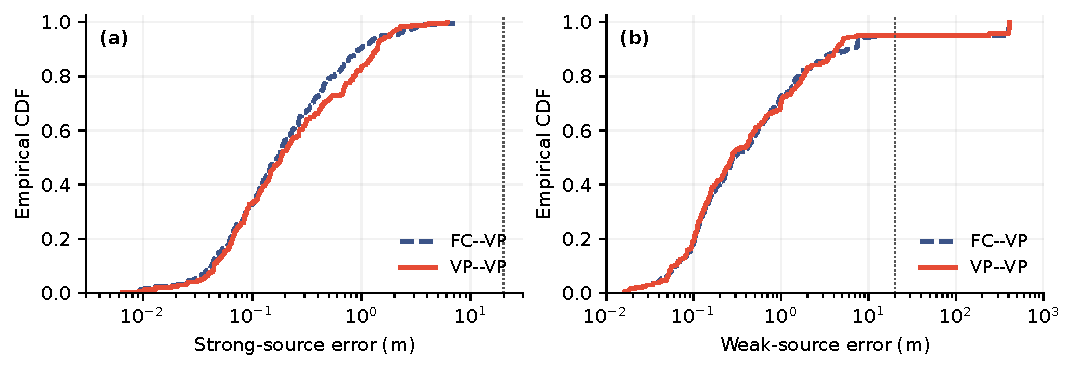
\includegraphics[width=\linewidth]{figures/error_cdf.pdf}
\caption{Matched-error empirical CDFs for all 240 curvature pairs. The dotted line marks 20 m. Logarithmic axes retain the full error range.}\label{fig:errors}
\end{figure}

Figure~\ref{fig:errors} shows similar error distributions, including the weak-source tail. The identical success decisions do not imply identical position estimates; the strong- and weak-source RMSEs differ slightly. Every observation contributes to the CDF and RMSE.

\begin{figure}[pos=H]
\centering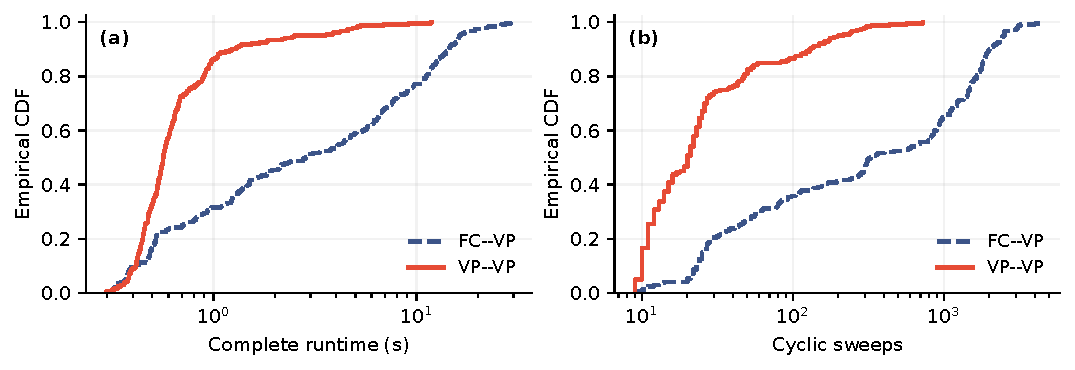
\includegraphics[width=\linewidth]{figures/cost_cdf.pdf}
\caption{Complete-runtime and cyclic-sweep CDFs for the same 240 pairs. All source-addition stages contribute to the cycle count.}\label{fig:cost}
\end{figure}

Figure~\ref{fig:cost} shows a shorter slow tail. Mean Newton attempts decrease from 1498.82 to 135.55, and cycles from 810.90 to 47.97; rejected directions remain in the count. VP--VP is faster in 170/240 cases, so the mean gain is particularly influenced by reductions in slow cases. Recording and final checks together average 0.0254/0.0059 s, much less than the 4.669 s time difference. Fewer updates and cycles support the curvature explanation in \eqref{eq:rate}.

Terminal quality is evaluated with the same full joint objective,
\begin{equation}
 J(\bm P)=E^{-1}\sum_f\|(I_L-\bm A_f\bm A_f^\dagger)\bm x_f\|^2,
 \quad \bm A_f=[\bm a_f(\bm p_1),\ldots,\bm a_f(\bm p_K)],
 \label{eq:joint}
\end{equation}
where $\bm P$ stacks all source coordinates and $\dagger$ denotes the pseudoinverse. Its bound-projected gradient is formed in metre coordinates by zeroing positive components at lower bounds and negative components at upper bounds. We report its infinity norm. VP--VP attains no higher $J$ in any pair: 199 reductions exceed $10^{-10}$ and 41 differences fall within this numerical tolerance. The projected-gradient median decreases from $2.03\times10^{-6}$ to $1.30\times10^{-7}$, and its P95 from $5.33\times10^{-6}$ to $1.79\times10^{-6}$; it is lower in every pair. Thus the computational savings do not accompany poorer terminal fitting or stationarity under the common energy stop. These measures do not certify global optimality or replace the localization errors.

\subsection{Small-step mechanism}
Formal trajectories clarify the iteration mechanism. For each observation, we divide accepted displacements below 0.01 m by all accepted updates, excluding rejections. The median fraction is 67.48\% for FC--VP and 65.74\% for VP--VP. Short steps are therefore common in both, consistent with the shared local-exit threshold; their fraction alone does not explain the saving. FC--VP accepts all 359,717 attempted updates without Hessian repair, capping, backtracking reduction or boundary clipping. Its short steps originate in the computed directions. After the second source is added, median cyclic sweeps decrease from 89.5 to 19, and P95 from 1647 to 197.85. The gain lies in fewer repeated cyclic refinements, rather than a uniform increase in step length. All fractions are summarized per observation before aggregation.

An earlier eight-observation diagnostic (four configurations, one realization and 0/15 dB gaps) uses FC--FC, with coefficients fixed for both the direction and acceptance, then refitted after acceptance. Of 21,436 accepted updates, 17,935 (83.67\%) are below 0.01 m, again without any of the four safeguards. This separate diagnostic supports the same direction-origin observation and is not pooled with the formal pairs.

\FloatBarrier
\subsection{Complete-locator test}
To examine the complete locator, methods frozen before testing are evaluated at 16 new source configurations, five realizations each and the same six gaps ($n=480$). Receiver coordinates remain unchanged. The alternating-projection references AP1/AP5 retain one/five peaks from a conditional projected-response score. Each position pair is continuously refined using the full two-source residual after joint coefficient elimination; the pair with the smallest final residual is returned. Both use projected-gradient tolerance $10^{-8}$.

Table~\ref{tab:results}B shows that both AP versions succeed throughout, while VP-BNOMP succeeds in 81.25\%. Its 90 failures concentrate in four configurations and are already present in the first saved complete two-source output. That output follows initial discovery and refinement, so it does not isolate which stage caused the failures. These results show that reducing local refinement cost alone does not resolve all configuration-dependent failures of the sequential locator.

\newpage
\begin{samepage}
\section{Conclusion}
Waveform elimination removes compensable position--coefficient coupling from the block-Newton curvature. The resulting frequency-wise update reduces repeated cyclic refinement while preserving residual-based discovery. Under common acceptance and stopping rules, the tested 240-observation comparison saves 83.77\% mean complete time with identical 20 m success decisions, similar error distributions and no deterioration in terminal joint fitting or stationarity. New-source-position tests show that local curvature improvement alone does not resolve configuration-dependent failures of the complete sequential locator. The interaction between source discovery and refinement remains a direction for further study.
\end{samepage}

% Funding and unconfirmed declarations remain blank, as requested.
\bibliographystyle{template/cas-model2-names}
\bibliography{references/references}
\end{document}
